\documentclass[12pt,a4paper]{article}

% ===== Codificación y español =====
\usepackage[utf8]{inputenc}
\usepackage[T1]{fontenc}
\usepackage[spanish, es-tabla]{babel}

% ===== Márgenes y gráficos =====
\usepackage{geometry}
\geometry{margin=2.5cm}
\usepackage{graphicx}
\usepackage{float}        % [H] para fijar figuras/tablas
\usepackage{subcaption}   % subfiguras
\usepackage{booktabs}     % tablas más bonitas

% ===== Hipervínculos y referencias =====
\usepackage{hyperref}
\hypersetup{
  colorlinks=true,
  linkcolor=black,
  citecolor=black,
  urlcolor=blue
}

\usepackage{siunitx}
\sisetup{
  output-decimal-marker = {.}, % decimal con punto
  group-separator = {,},       % miles con coma
  group-minimum-digits = 4,
  group-digits = integer,
  table-number-alignment = center,
  round-mode = places,
  detect-all = true            % ignora configuraciones de babel
}

% Ayuda al manejo de tablas
\usepackage{tabularx}
\usepackage{adjustbox}
\usepackage{longtable}

% cleveref mejora \ref: escribe "Figura 1", "Tabla 2", etc.
\usepackage[capitalise,noabbrev]{cleveref}

% Ajuste de nombres en cleveref
\crefname{figure}{figura}{figuras}
\Crefname{figure}{Figura}{Figuras}
\crefname{subfigure}{subfigura}{subfiguras}
\Crefname{subfigure}{Subfigura}{Subfiguras}
\crefname{table}{tabla}{tablas}
\Crefname{table}{Tabla}{Tablas}
\crefname{equation}{ecuación}{ecuaciones}
\Crefname{equation}{Ecuación}{Ecuaciones}
\crefname{section}{sección}{secciones}
\Crefname{section}{Sección}{Secciones}

% Listas más controlables
\usepackage{enumitem}

\graphicspath{{figures/}}

% ===== Título y autoría =====
\title{\textbf{\textit{"Playing"} con diferentes clasificadores y datasets}}
\author{Haessler Joan Ortiz Moncada \\[0.5cm]
        Universidad Distrital Francisco José de Caldas \\
        Facultad de Ingeniería \\
        Curso: Big Data}
\date{\today}

\begin{document}

\maketitle

\section{Introducción}
Este documento presenta el desarrollo del \texttt{Assignment \#4} del curso de Big Data y documenta 
los hallazgos y análisis correspondientes, haciendo uso de tres métricas e incorporando gráficos 
adecuados que permitan evidenciar y sustentar los resultados. El \texttt{Assignment \#4} propone 
experimentar con diversos modelos de clasificación sobre distintos conjuntos de datos (\texttt{Blobs}, 
\texttt{Gaussian Quartiles} y \texttt{Moons}), con diferentes tamaños de muestra y niveles de ruido 
inducido.

\section{Metodología}
Se desarrolla conforme a lo establecido en el \texttt{Assignment \#4}, aunque con algunas variaciones 
en la presentación. En aquel caso se solicitaba que todo el trabajo se realizara en un único documento o 
archivo de Colab; en cambio, aquí se optó por efectuar la codificación en dicho entorno y presentar los 
hallazgos y el compendio de resultados mediante un informe escrito. Se emplearon principalmente Google Colab y Python, 
haciendo uso de los paquetes \texttt{os}, \texttt{pandas}, \texttt{scikit-learn}, \texttt{matplotlib} y \texttt{seaborn}.
También se tuvo en cuenta manejar el mismo escenario de aleatoriedad (semiila) para poder replicar los resultados.

Básicamente, lo que se hizo fue ir desarrollando en Colab el código correspondiente y de manera 
paralela documentar los hallazgos y resultados en este informe. El archivo de este informe se encuentran en la carpeta taller\_4 del repositorio de 
GitHub \href{https://github.com/HaesslerOrtiz/bigdata}{bigdata\_repositorio}.

\section{Escenario 1: binario vs. clasificación multiclase}
En esta sección se construyeron tres conjuntos de datos: uno binario (dos clases) y otros dos con cinco y veinte clases, 
respectivamente. Como el \texttt{Assignment \#4} no especificó el tamaño, se fijaron en 1,000 registros cada uno. Para 
su construcción se emplearon datos tipo \texttt{Blobs}, cuyas observaciones se distribuyen como puntos en el plano 
cartesiano; cada clase agrupa sus puntos en una región del espacio. Los datos se dividieron en entrenamiento, validación 
y prueba en proporciones de 60\%, 20\% y 20\%, respectivamente; además, se aplicó estratificación para que cada partición 
mantuviera la misma distribución de clases que el dataset padre. La \Cref{fig:hist_2_5} muestra como las frecuencias 
de las clases para el dataset binario y para el de cinco clases, mientras la \Cref{fig:hist_20} muestra la frecuencia 
del dataset que cse clasifica en 20 clases.

\begin{figure}[H]
  \centering
  \begin{subfigure}[b]{0.45\textwidth}
    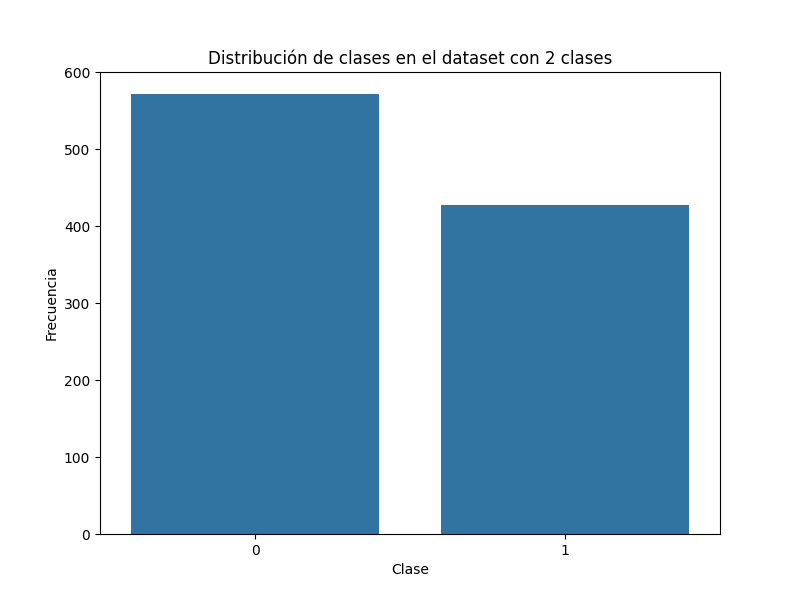
\includegraphics[width=\textwidth]{histogram_2_classes.png}
    \caption{Frecuencia clases dataset binario.}
    \label{fig:hist_2}
  \end{subfigure}
  \hfill
  \begin{subfigure}[b]{0.45\textwidth}
    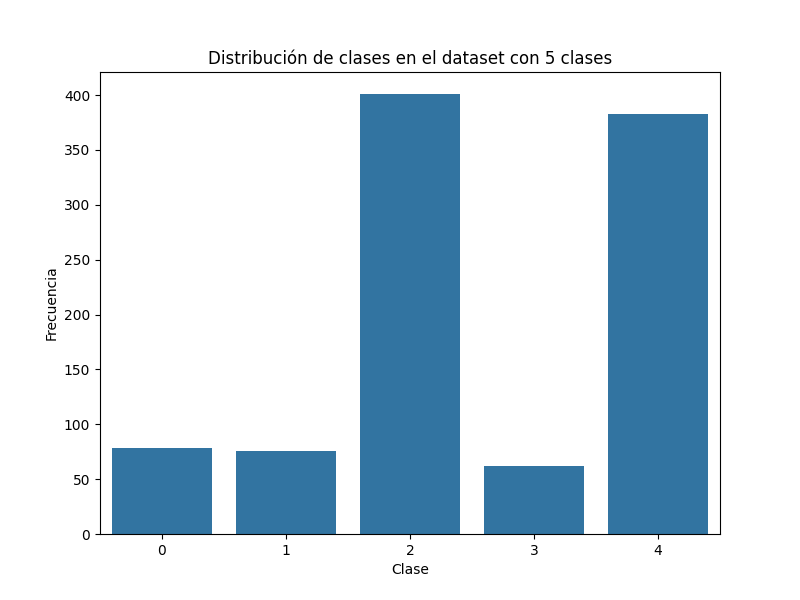
\includegraphics[width=\textwidth]{histogram_5_classes.png}
    \caption{Frecuencia clases dataset de cinco clases.}
    \label{fig:hist_5}
  \end{subfigure}
  \caption{Frecuencia clases datasets binario y de cinco clases.}
  \label{fig:hist_2_5}
\end{figure}

\begin{figure}[H]
  \centering
  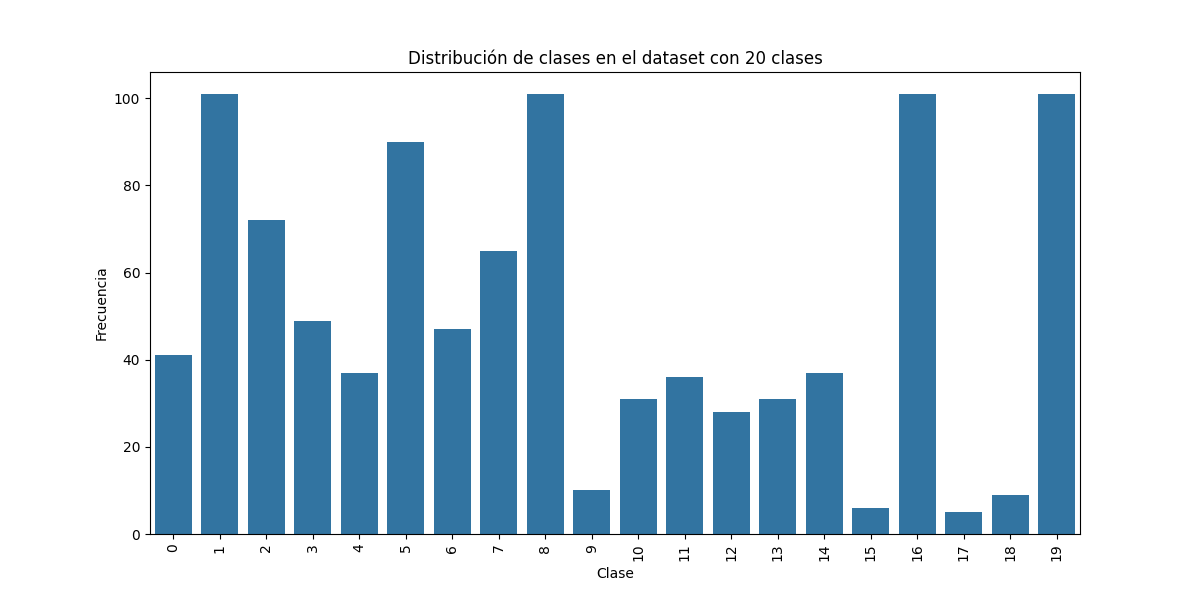
\includegraphics[width=\textwidth]{histogram_20_classes.png}
  \caption{Frecuencia clases dataset de veinte clases.}
  \label{fig:hist_20}
\end{figure}

\subsection{Probando con distintos clasificadores}
En este y en los siguientes escenarios, se evaluará cómo distintos clasificadores predicen las clases de cada conjunto de datos, 
explorando los hiperparámetros configurables de cada modelo. Posteriormente, se seleccionará la combinación de hiperparámetros 
que ofrezca el mejor desempeño predictivo según las métricas \texttt{Accuracy}, \texttt{Recall} y \texttt{F1-Score}. Cabe acalarar 
que fue con el conjunto de validación con el que se encontraron los mejores hiperparámetros en todos los escenarios y para todos 
los modelos.

\begin{enumerate}

  \item \textbf{Vecinos más cercanos (k-NN).}
  Probando con un rango de 1 a 30 vecinos para cada uno de los datasets conformados, se definio que el mejor desempeño se obtuvo 
  con los siguientes hiperparámetros:

  \begin{itemize}
    \item \textbf{Dataset binario.} 1 vecinos.
    \item \textbf{Dataset con cinco clases.} 8 vecinos.
    \item \textbf{Dataset con veinte clases.} 19 vecinos.
  \end{itemize}

  Respecto al desempeño obtenido en cada uno de los modelos se tienen los siguientes resultados:

  \small
  \setlength{\tabcolsep}{4pt}
  \begin{longtable}{@{}lcccc@{}}
    \toprule
    \textbf{Clase} & \textbf{Precision} & \textbf{Recall} & \textbf{F1-Score} & \textbf{Support} \\
    \midrule
    \endfirsthead

    \toprule
    \textbf{Clase} & \textbf{Precision} & \textbf{Recall} & \textbf{F1-Score} & \textbf{Support} \\
    \midrule
    \endhead

    \midrule
    \multicolumn{5}{r}{\emph{Continúa en la siguiente página}} \\
    \endfoot

    \bottomrule
    \caption{Reportes de clasificación k-NN SC1.}
    \label{tab:reportes_clasificacion_knn_sc1}
    \endlastfoot

    % ================= (a) 2 clases =================
    \multicolumn{5}{@{}l}{\textbf{(a) 2 clases}}\\
    0 & 1.00 & 1.00 & 1.00 & 115 \\
    1 & 1.00 & 1.00 & 1.00 & 85 \\
    \midrule
    \multicolumn{3}{l}{\textbf{Accuracy}} & \textbf{1.00} & 200 \\
    \textbf{Macro avg}    & 1.00 & 1.00 & 1.00 & 200 \\
    \textbf{Weighted avg} & 1.00 & 1.00 & 1.00 & 200 \\
    \addlinespace[0.8em]

    % ================= (b) 5 clases =================
    \multicolumn{5}{@{}l}{\textbf{(b) 5 clases}}\\
    0 & 1.00 & 1.00 & 1.00 & 16 \\
    1 & 0.86 & 0.80 & 0.83 & 15 \\
    2 & 1.00 & 1.00 & 1.00 & 80 \\
    3 & 1.00 & 1.00 & 1.00 & 13 \\
    4 & 0.96 & 0.97 & 0.97 & 76 \\
    \midrule
    \multicolumn{3}{l}{\textbf{Accuracy}} & \textbf{0.97} & 200 \\
    \textbf{Macro avg}    & 0.96 & 0.95 & 0.96 & 200 \\
    \textbf{Weighted avg} & 0.97 & 0.97 & 0.97 & 200 \\
    \addlinespace[0.8em]

    % ================= (c) 20 clases =================
    \multicolumn{5}{@{}l}{\textbf{(c) 20 clases}}\\
    0 & 1.00 & 1.00 & 1.00 & 8 \\
    1 & 0.91 & 1.00 & 0.95 & 20 \\
    2 & 0.67 & 0.53 & 0.59 & 15 \\
    3 & 0.80 & 0.40 & 0.53 & 10 \\
    4 & 1.00 & 1.00 & 1.00 & 7 \\
    5 & 0.52 & 0.67 & 0.59 & 18 \\
    6 & 1.00 & 1.00 & 1.00 & 9 \\
    7 & 0.56 & 0.77 & 0.65 & 13 \\
    8 & 0.83 & 1.00 & 0.91 & 20 \\
    9 & 0.00 & 0.00 & 0.00 & 2 \\
    10 & 0.75 & 1.00 & 0.86 & 6 \\
    11 & 0.71 & 0.71 & 0.71 & 7 \\
    12 & 1.00 & 1.00 & 1.00 & 6 \\
    13 & 0.75 & 0.50 & 0.60 & 6 \\
    14 & 1.00 & 0.88 & 0.93 & 8 \\
    15 & 0.00 & 0.00 & 0.00 & 1 \\
    16 & 0.65 & 0.65 & 0.65 & 20 \\
    17 & 0.00 & 0.00 & 0.00 & 1 \\
    18 & 0.00 & 0.00 & 0.00 & 2 \\
    19 & 1.00 & 0.95 & 0.98 & 21 \\
    \midrule
    \multicolumn{3}{l}{\textbf{Accuracy}} & \textbf{0.79} & 200 \\
    \textbf{Macro avg}    & 0.66 & 0.65 & 0.65 & 200 \\
    \textbf{Weighted avg} & 0.78 & 0.79 & 0.78 & 200 \\
  \end{longtable}

  \item \textbf{Arbol de decisión.}
  Se buscó la mejor configuración de hiperparámetros en el siguiente marco:
  \begin{table}[htbp]
    \centering
    \begin{tabular}{@{}lll@{}}
      \toprule
      \textbf{Parámetro} & \textbf{Descripción} & \textbf{Valores probados} \\
      \midrule
      \texttt{max\_depth} & Profundidad máxima del árbol & \{None, 5, 10, 15, 20\} \\
      \texttt{min\_samples\_split} & Mín. muestras para dividir un nodo interno & \{2, 5, 10\} \\
      \texttt{min\_samples\_leaf} & Mín. muestras por hoja & \{1, 2, 4\} \\
      \bottomrule
    \end{tabular}
    \caption{Busqueda de hiperparámetros Arbol de de Decisión SC1.}
    \label{tab:param_dt_sc1}
  \end{table}

  Con base en esta busqueda se obtuvieron las siguientes mejores configuraciones de hiperparámetros para cada dataset:

  \begin{table}[htbp]
    \centering
    \begin{tabular}{@{}lccc@{}}
      \toprule
      \textbf{Clases} & \texttt{max\_depth} & \texttt{min\_samples\_leaf} & \texttt{min\_samples\_split} \\
      \midrule
      2  & \texttt{None} & 1 & 2 \\
      5  & 5              & 1 & 2 \\
      20 & 10             & 1 & 5 \\
      \bottomrule
    \end{tabular}
    \caption{Mejores hiperparámetros encontrados para Árbol de decisión SC1.}
    \label{tab:best_hparams_dt_sc1}
  \end{table}

  Respecto al desempeño obtenido en cada uno de los modelos se tienen los siguientes resultados:

  \small
  \setlength{\tabcolsep}{4pt}
  \begin{longtable}{@{}lcccc@{}}
    \toprule
    \textbf{Clase} & \textbf{Precision} & \textbf{Recall} & \textbf{F1-Score} & \textbf{Support} \\
    \midrule
    \endfirsthead

    \toprule
    \textbf{Clase} & \textbf{Precision} & \textbf{Recall} & \textbf{F1-Score} & \textbf{Support} \\
    \midrule
    \endhead

    \midrule
    \multicolumn{5}{r}{\emph{Continúa en la siguiente página}} \\
    \endfoot

    \bottomrule
    \caption{Reportes de clasificación Árbol de decisión SC1.}
    \label{tab:reportes_dt_sc1}
    \endlastfoot

    % ================= (a) 2 clases =================
    \multicolumn{5}{@{}l}{\textbf{(a) 2 clases}}\\
    0 & 1.00 & 1.00 & 1.00 & 115 \\
    1 & 1.00 & 1.00 & 1.00 & 85 \\
    \midrule
    \multicolumn{3}{l}{\textbf{Accuracy}} & \textbf{1.00} & 200 \\
    \textbf{Macro avg}    & 1.00 & 1.00 & 1.00 & 200 \\
    \textbf{Weighted avg} & 1.00 & 1.00 & 1.00 & 200 \\
    \addlinespace[0.8em]

    % ================= (b) 5 clases =================
    \multicolumn{5}{@{}l}{\textbf{(b) 5 clases}}\\
    0 & 1.00 & 1.00 & 1.00 & 16 \\
    1 & 0.71 & 0.67 & 0.69 & 15 \\
    2 & 1.00 & 1.00 & 1.00 & 80 \\
    3 & 1.00 & 1.00 & 1.00 & 13 \\
    4 & 0.94 & 0.95 & 0.94 & 76 \\
    \midrule
    \multicolumn{3}{l}{\textbf{Accuracy}} & \textbf{0.95} & 200 \\
    \textbf{Macro avg}    & 0.93 & 0.92 & 0.93 & 200 \\
    \textbf{Weighted avg} & 0.95 & 0.95 & 0.95 & 200 \\
    \addlinespace[0.8em]

    % ================= (c) 20 clases =================
    \multicolumn{5}{@{}l}{\textbf{(c) 20 clases}}\\
    0 & 1.00 & 0.88 & 0.93 & 8 \\
    1 & 0.91 & 1.00 & 0.95 & 20 \\
    2 & 0.53 & 0.60 & 0.56 & 15 \\
    3 & 0.80 & 0.40 & 0.53 & 10 \\
    4 & 1.00 & 1.00 & 1.00 & 7 \\
    5 & 0.50 & 0.72 & 0.59 & 18 \\
    6 & 1.00 & 1.00 & 1.00 & 9 \\
    7 & 0.46 & 0.46 & 0.46 & 13 \\
    8 & 0.91 & 1.00 & 0.95 & 20 \\
    9 & 1.00 & 0.50 & 0.67 & 2 \\
    10 & 0.75 & 1.00 & 0.86 & 6 \\
    11 & 1.00 & 0.86 & 0.92 & 7 \\
    12 & 0.86 & 1.00 & 0.92 & 6 \\
    13 & 0.80 & 0.67 & 0.73 & 6 \\
    14 & 1.00 & 0.88 & 0.93 & 8 \\
    15 & 0.00 & 0.00 & 0.00 & 1 \\
    16 & 0.76 & 0.65 & 0.70 & 20 \\
    17 & 1.00 & 1.00 & 1.00 & 1 \\
    18 & 1.00 & 0.50 & 0.67 & 2 \\
    19 & 1.00 & 0.81 & 0.89 & 21 \\
    \midrule
    \multicolumn{3}{l}{\textbf{Accuracy}} & \textbf{0.79} & 200 \\
    \textbf{Macro avg}    & 0.81 & 0.75 & 0.76 & 200 \\
    \textbf{Weighted avg} & 0.81 & 0.79 & 0.79 & 200 \\
  \end{longtable}

  \item \textbf{Máquinas de vectores de soporte (SVM por sus siglas en inglés).}
  Para este clasificador se buscó la mejor configuración de hiperparámetros probando los siguientes valores:

  \begin{table}[htbp]
    \centering
    \begin{tabular}{@{}lll@{}}
      \toprule
      \textbf{Parámetro} & \textbf{Descripción} & \textbf{Valores probados} \\
      \midrule
      \texttt{C} & Parámetro de regularización. & \{0.1, 1, 10\} \\
      \texttt{kernel} & Tipo de núcleo usado por el algoritmo SVM. & \{\texttt{linear}, \texttt{rbf}\} \\
      \texttt{gamma} & Coeficiente del kernel. & \{\texttt{scale}, \texttt{auto}, 0.1, 1\} \\
      \bottomrule
    \end{tabular}
    \caption{Busqueda de hiperparámetros para SVM SC1.}
    \label{tab:param_svm_sc1}
  \end{table}
  
  Los mejores hiperparámetros encontrados para cada dataset, fueron los siguientes:

  \begin{table}[H]
    \centering
    \begin{tabular}{@{}lccc@{}}
      \toprule
      \textbf{Clases} & \texttt{C} & \texttt{gamma} & \texttt{kernel} \\
      \midrule
      2  & 0.1 & \texttt{scale} & \texttt{linear} \\
      5  & 0.1 & \texttt{scale} & \texttt{linear} \\
      20 & 0.1 & \texttt{scale} & \texttt{linear} \\
      \bottomrule
    \end{tabular}
    \caption{Mejores hiperparámetros SVM SC1.}
    \label{tab:best_hparams_svm_sc1}
  \end{table}
  
  Con los mejores hiperparámetros encontrados, se obtuvieron los siguientes resultados:

  \small
  \setlength{\tabcolsep}{4pt}
  \begin{longtable}{@{}lcccc@{}}
    \toprule
    \textbf{Clase} & \textbf{Precision} & \textbf{Recall} & \textbf{F1-Score} & \textbf{Support} \\
    \midrule
    \endfirsthead

    \toprule
    \textbf{Clase} & \textbf{Precision} & \textbf{Recall} & \textbf{F1-Score} & \textbf{Support} \\
    \midrule
    \endhead

    \midrule
    \multicolumn{5}{r}{\emph{Continúa en la siguiente página}} \\
    \endfoot

    \bottomrule
    \caption{Reportes de clasificación SVM SC1.}
    \label{tab:reportes_clasificacion_svm}
    \endlastfoot

    % ================= (a) 2 clases =================
    \multicolumn{5}{@{}l}{\textbf{(a) 2 clases}}\\
    0 & 1.00 & 1.00 & 1.00 & 115 \\
    1 & 1.00 & 1.00 & 1.00 & 85 \\
    \midrule
    \multicolumn{3}{l}{\textbf{Accuracy}} & \textbf{1.00} & 200 \\
    \textbf{Macro avg}    & 1.00 & 1.00 & 1.00 & 200 \\
    \textbf{Weighted avg} & 1.00 & 1.00 & 1.00 & 200 \\
    \addlinespace[0.8em]

    % ================= (b) 5 clases =================
    \multicolumn{5}{@{}l}{\textbf{(b) 5 clases}}\\
    0 & 1.00 & 1.00 & 1.00 & 16 \\
    1 & 0.86 & 0.80 & 0.83 & 15 \\
    2 & 1.00 & 1.00 & 1.00 & 80 \\
    3 & 1.00 & 1.00 & 1.00 & 13 \\
    4 & 0.96 & 0.97 & 0.97 & 76 \\
    \midrule
    \multicolumn{3}{l}{\textbf{Accuracy}} & \textbf{0.97} & 200 \\
    \textbf{Macro avg}    & 0.96 & 0.95 & 0.96 & 200 \\
    \textbf{Weighted avg} & 0.97 & 0.97 & 0.97 & 200 \\
    \addlinespace[0.8em]

    % ================= (c) 20 clases =================
    \multicolumn{5}{@{}l}{\textbf{(c) 20 clases}}\\
    0 & 1.00 & 1.00 & 1.00 & 8 \\
    1 & 0.95 & 1.00 & 0.98 & 20 \\
    2 & 0.60 & 0.60 & 0.60 & 15 \\
    3 & 0.80 & 0.40 & 0.53 & 10 \\
    4 & 1.00 & 1.00 & 1.00 & 7 \\
    5 & 0.53 & 0.56 & 0.54 & 18 \\
    6 & 1.00 & 1.00 & 1.00 & 9 \\
    7 & 0.57 & 0.62 & 0.59 & 13 \\
    8 & 0.91 & 1.00 & 0.95 & 20 \\
    9 & 1.00 & 1.00 & 1.00 & 2 \\
    10 & 0.75 & 1.00 & 0.86 & 6 \\
    11 & 1.00 & 0.71 & 0.83 & 7 \\
    12 & 1.00 & 1.00 & 1.00 & 6 \\
    13 & 0.83 & 0.83 & 0.83 & 6 \\
    14 & 1.00 & 0.88 & 0.93 & 8 \\
    15 & 0.00 & 0.00 & 0.00 & 1 \\
    16 & 0.58 & 0.70 & 0.64 & 20 \\
    17 & 1.00 & 1.00 & 1.00 & 1 \\
    18 & 1.00 & 0.50 & 0.67 & 2 \\
    19 & 1.00 & 0.95 & 0.98 & 21 \\
    \midrule
    \multicolumn{3}{l}{\textbf{Accuracy}} & \textbf{0.81} & 200 \\
    \textbf{Macro avg}    & 0.83 & 0.79 & 0.80 & 200 \\
    \textbf{Weighted avg} & 0.82 & 0.81 & 0.81 & 200 \\
  \end{longtable}

   \item \textbf{Perceptrón multicapa (MLP por sus siglas en inglés).}
   Para este clasificador se buscó la mejor configuración de hiperparámetros probando con los siguientes valores:

   \begin{table}[htbp]
    \centering\small
    \setlength{\tabcolsep}{4pt}
    \begin{tabularx}{\linewidth}{@{}l l X@{}}
      \toprule
      \textbf{Parámetro} & \textbf{Descripción} & \textbf{Valores probados} \\
      \midrule
      \texttt{hidden\_layer\_sizes} & Tamaño(s) de capa(s) oculta(s) & \texttt{(50,)}, \texttt{(100,)}, \texttt{(50, 50)} \\
      \texttt{activation}           & Función de activación          & \texttt{tanh}, \texttt{relu} \\
      \texttt{solver}               & Optimizador para los pesos     & \texttt{adam} \\
      \texttt{alpha}                & Regularización L2              & 0.0001, 0.001 \\
      \texttt{learning\_rate\_init} & Tasa de aprendizaje inicial    & 0.001, 0.01 \\
      \texttt{max\_iter}            & Iteraciones máximas            & 200, 500 \\
      \bottomrule
    \end{tabularx}
    \caption{Busqueda de hiperparámetros para MLP SC1.}
    \label{tab:param_mlp_sc1}
  \end{table}

   Solo se usó un solo optimizador de pesos, conforme lo sugirió la IA de Colab. Con base en esta busqueda se obtuvieron 
   las siguientes mejores configuraciones de hiperparámetros para cada dataset:

  \begin{table}[htbp]
    \centering\small
    \setlength{\tabcolsep}{4pt}
    \begin{tabularx}{\linewidth}{@{}l l l l l l l@{}}
      \toprule
      \textbf{Clases} & \textbf{\texttt{hidden\_layer\_sizes}} & \textbf{\texttt{activation}} & \textbf{\texttt{solver}} & \textbf{\texttt{alpha}} & \textbf{\texttt{learning\_rate\_init}} & \textbf{\texttt{max\_iter}} \\
      \midrule
      2  & \texttt{(50,)}     & \texttt{tanh} & \texttt{adam} & 0.0001 & 0.001 & 200 \\
      5  & \texttt{(50, 50)}  & \texttt{tanh} & \texttt{adam} & 0.0001 & 0.01  & 200 \\
      20 & \texttt{(100,)}    & \texttt{tanh} & \texttt{adam} & 0.0001 & 0.001 & 500 \\
      \bottomrule
    \end{tabularx}
    \caption{Mejores hiperparámetros MLP SC1.}
    \label{tab:best_hparams_mlp_SC1}
  \end{table}

   Con la configuraciones de hiperparámetros encontradas, se obtuvieron los siguientes resultados:

    \small
    \setlength{\tabcolsep}{4pt}
    \begin{longtable}{@{}lcccc@{}}
      \toprule
      \textbf{Clase} & \textbf{Precision} & \textbf{Recall} & \textbf{F1-Score} & \textbf{Support} \\
      \midrule
      \endfirsthead

      \toprule
      \textbf{Clase} & \textbf{Precision} & \textbf{Recall} & \textbf{F1-Score} & \textbf{Support} \\
      \midrule
      \endhead

      \midrule
      \multicolumn{5}{r}{\emph{Continúa en la siguiente página}} \\
      \endfoot

      \bottomrule
      \caption{Reportes de clasificación MLP SC1.}
      \label{tab:mlp_reports_long}
      \endlastfoot

      % ================= (a) 2 clases =================
      \multicolumn{5}{@{}l}{\textbf{(a) 2 clases}}\\
      0 & 1.00 & 1.00 & 1.00 & 115 \\
      1 & 1.00 & 1.00 & 1.00 & 85 \\
      \midrule
      \multicolumn{3}{l}{\textbf{Accuracy}} & \textbf{1.00} & 200 \\
      \textbf{Macro avg}    & 1.00 & 1.00 & 1.00 & 200 \\
      \textbf{Weighted avg} & 1.00 & 1.00 & 1.00 & 200 \\
      \addlinespace[0.8em]

      % ================= (b) 5 clases =================
      \multicolumn{5}{@{}l}{\textbf{(b) 5 clases}}\\
      0 & 1.00 & 1.00 & 1.00 & 16 \\
      1 & 0.86 & 0.80 & 0.83 & 15 \\
      2 & 1.00 & 1.00 & 1.00 & 80 \\
      3 & 1.00 & 1.00 & 1.00 & 13 \\
      4 & 0.96 & 0.97 & 0.97 & 76 \\
      \midrule
      \multicolumn{3}{l}{\textbf{Accuracy}} & \textbf{0.97} & 200 \\
      \textbf{Macro avg}    & 0.96 & 0.95 & 0.96 & 200 \\
      \textbf{Weighted avg} & 0.97 & 0.97 & 0.97 & 200 \\
      \addlinespace[0.8em]

      % ================= (c) 20 clases =================
      \multicolumn{5}{@{}l}{\textbf{(c) 20 clases}}\\
      0 & 1.00 & 1.00 & 1.00 & 8 \\
      1 & 0.95 & 1.00 & 0.98 & 20 \\
      2 & 0.60 & 0.60 & 0.60 & 15 \\
      3 & 0.75 & 0.60 & 0.67 & 10 \\
      4 & 1.00 & 1.00 & 1.00 & 7 \\
      5 & 0.56 & 0.56 & 0.56 & 18 \\
      6 & 1.00 & 1.00 & 1.00 & 9 \\
      7 & 0.57 & 0.62 & 0.59 & 13 \\
      8 & 0.95 & 1.00 & 0.98 & 20 \\
      9 & 1.00 & 1.00 & 1.00 & 2 \\
      10 & 0.75 & 1.00 & 0.86 & 6 \\
      11 & 1.00 & 0.86 & 0.92 & 7 \\
      12 & 1.00 & 1.00 & 1.00 & 6 \\
      13 & 0.83 & 0.83 & 0.83 & 6 \\
      14 & 1.00 & 0.88 & 0.93 & 8 \\
      15 & 0.00 & 0.00 & 0.00 & 1 \\
      16 & 0.59 & 0.65 & 0.62 & 20 \\
      17 & 1.00 & 1.00 & 1.00 & 1 \\
      18 & 1.00 & 0.50 & 0.67 & 2 \\
      19 & 1.00 & 0.95 & 0.98 & 21 \\
      \midrule
      \multicolumn{3}{l}{\textbf{Accuracy}} & \textbf{0.82} & 200 \\
      \textbf{Macro avg}    & 0.83 & 0.80 & 0.81 & 200 \\
      \textbf{Weighted avg} & 0.82 & 0.82 & 0.82 & 200 \\
    \end{longtable}

  \item \textbf{Análisis de resultados.}
  
  \begin{itemize}
    \item \textbf{Tendencia general.} Con 2 clases, todos los modelos aciertan casi perfecto. Con 5 clases siguen muy altos. 
    Al pasar a \textbf{20 clases}, la exactitud baja para todos ($\approx$ 0.79--0.82) por mayor solapamiento entre clases 
    y menos ejemplos por clase.
    
    \item \textbf{K-NN.} Excelente con pocas clases, pero cae más con 20 clases: encontrar vecinos “correctos” se vuelve 
    difícil en un espacio de variables fijo.
    
    \item \textbf{Árbol de decisión.} También disminuye con más clases. Al dividir con cortes alineados a ejes, requiere 
    muchos \emph{splits} y puede sobreajustar cuando hay pocos datos por clase.
    
    \item \textbf{SVM.} Con 2 y 5 clases, el \emph{kernel} lineal funciona muy bien (clases bastante separables). Con 20 
    clases suele requerir \emph{RBF} para fronteras no lineales y se mantiene competitivo.
    
    \item \textbf{MLP.} Rinde muy bien en general. Con 20 clases suele estar entre los mejores; puede necesitar redes más 
    grandes y más iteraciones para converger.
    
    \item \textbf{“Mejor” por conjunto.} 
    \begin{itemize}
      \item \textbf{2 clases:} todos al tope ($\approx$ 1.00).
      \item \textbf{5 clases:} K-NN y SVM lideran; Árbol y MLP muy cerca.
      \item \textbf{20 clases:} MLP o K-NN encabezan según el corrido; diferencias pequeñas ($\approx$ 0.79--0.82).
    \end{itemize}
    
    \item \textbf{Variabilidad por clase (20 clases).} Se observan clases minoritarias con precisión/recall/f1 bajos e incluso 
    métricas indefinidas cuando no se predice alguna clase, lo que apunta a \textbf{desbalance} y \textbf{solapamiento} entre clases.
  \end{itemize}

  \paragraph{Posibles mejoras en la predicción del dataset de 20 clases}
  \begin{enumerate}
    \item Tratar el \textbf{desbalance} (pesos por clase, sobremuestreo/SMOTE).
    \item \textbf{Ampliar y afinar} hiperparámetros: $k$ en K-NN; poda/profundidad en Árbol; $C$ y $\gamma$ en SVM; capas, 
    neuronas, iteraciones y \emph{early stopping} en MLP.
    \item \textbf{Enriquecer las características} o transformar las actuales para mejorar la separabilidad.
    \item Probar \textbf{ensambles} (bagging/boosting) y \textbf{calibración} de probabilidades.
  \end{enumerate}

  \noindent En resumen, con pocas clases, casi todo funciona perfecto, con 20 clases, la tarea se complica y destacan los modelos 
  que aprenden \textbf{fronteras no lineales} y manejan mejor el \textbf{desbalance} (MLP/SVM), aunque K-NN puede empatar cuando las 
  clases quedan bien definidas.

  Adicionlmente el gráfico mostrado en la \Cref{fig:matriz_4x3} a continuación, permite visualizar como se trazaron 
  los diferentes límites de clasificación definidos pr cada modelo y para cada dataset.

  % ==== MACRO PARA UNA FILA DE 3 SUBFIGURAS (se adapta al ancho de la página) ====
  \newcommand{\threefigsrow}[3]{%
    \begin{subfigure}{0.32\textwidth}
      \centering
      \includegraphics[width=\linewidth]{#1}% <-- reemplaza con tu imagen
      \caption{}% <-- escribe el subtítulo (opcional)
    \end{subfigure}\hfill
    \begin{subfigure}{0.32\textwidth}
      \centering
      \includegraphics[width=\linewidth]{#2}
      \caption{}
    \end{subfigure}\hfill
    \begin{subfigure}{0.32\textwidth}
      \centering
      \includegraphics[width=\linewidth]{#3}
      \caption{}
    \end{subfigure}\par\medskip
  }

  % ==== MATRIZ DE 4x3 (3 por fila, 4 filas). SE PUEDE EXTENDER A MÁS DE UNA PÁGINA ====
  % Usa dos (o más) entornos figure con \ContinuedFloat para permitir salto de página
  \begin{figure}[h]
    \centering
    % ----- Fila 1 -----
    \threefigsrow{knn_decision_boundary_2_classes.png}{knn_decision_boundary_5_classes.png}{knn_decision_boundary_20_classes.png}
    % ----- Fila 2 -----
    \threefigsrow{dt_decision_boundary_2_classes.png}{dt_decision_boundary_5_classes.png}{dt_decision_boundary_20_classes.png}

    \caption{Matriz de fronteras de decisión.}% <- título general (parte 1)
    \label{fig:matriz_4x3}
  \end{figure}

  \begin{figure}[h]\ContinuedFloat
    \centering
    % ----- Fila 3 -----
    \threefigsrow{svm_decision_boundary_2_classes.png}{svm_decision_boundary_5_classes.png}{svm_decision_boundary_20_classes.png}
    % ----- Fila 4 -----
    \threefigsrow{mlp_decision_boundary_2_classes.png}{mlp_decision_boundary_5_classes.png}{mlp_decision_boundary_20_classes.png}
    \caption{Matriz de fronteras de decisión SC1.}% <- título general (parte 2)
    \label{fig:matriz_4x3}
  \end{figure}

\end{enumerate}

\section{Escenario 2: grandes datasets vs pequeños datasets}

Este escenario aborda un desarrollo muy similar al del anterior: se construyen conjuntos de datos, se dividen en subconjuntos de entrenamiento, 
validación y prueba, conservando la proporción de clases de los datasets originales y conservando la proporción del escenario anterior, 
y posteriormente se implementan los mismos modelos de clasificación del escenario previo. La diferencia principal radica en la forma de construir 
los conjuntos de datos: aquí los datos son de tipo \texttt{Quartiles Gaussian}; cada conjunto tiene cuatro clases y se generan cinco datasets 
con los siguientes tamaños: \(10^2,\,10^3,\,10^4,\,10^5,\,10^6\). A diferencia del anterior escenario, aquí si se va a generar la misma cantidad de 
registros para cada clase en cada dataset.

\begin{enumerate}
  \item \textbf{Vecinos más cercanos (k-NN).}
  Probando con un rango de 1 a 30 vecinos (al igual que en el anterior escenario) para cada uno de los datasets conformados, se obtuvo que el mejor 
  desempeño para todos los datasets fue con el número de vecinos igual a 1. Los resultados obtenidos fueron los siguientes:
  
  \small
  \setlength{\tabcolsep}{4pt}
  \begin{longtable}{@{}l l c c c r@{}}
    \toprule
    \textbf{Tamaño (muestras)} & \textbf{Línea} & \textbf{Precision} & \textbf{Recall} & \textbf{F1-score} & \textbf{Support} \\
    \midrule
    \endfirsthead

    \toprule
    \textbf{Tamaño (muestras)} & \textbf{Línea} & \textbf{Precision} & \textbf{Recall} & \textbf{F1-score} & \textbf{Support} \\
    \midrule
    \endhead

    \midrule
    \multicolumn{6}{r}{\emph{Continúa en la siguiente página}} \\
    \endfoot

    \bottomrule
    \caption{K-NN: métricas.}
    \label{tab:reportes_clasificacion_knn_sc2}
    \endlastfoot

    % ===== 100 samples =====
    100   & Clase 0       & 0.67 & 0.80 & 0.73 & 5 \\
          & Clase 1       & 0.33 & 0.20 & 0.25 & 5 \\
          & Clase 2       & 0.36 & 0.80 & 0.50 & 5 \\
          & Clase 3       & 0.00 & 0.00 & 0.00 & 5 \\
          & \textbf{Accuracy}    & \textbf{—}   & \textbf{—}   & \textbf{0.45} & \textbf{20} \\
          & Macro avg     & 0.34 & 0.45 & 0.37 & 20 \\
          & Weighted avg  & 0.34 & 0.45 & 0.37 & 20 \\
    \addlinespace

    % ===== 1,000 samples =====
    1\,000 & Clase 0      & 0.98 & 0.94 & 0.96 & 50 \\
          & Clase 1       & 0.90 & 0.86 & 0.88 & 50 \\
          & Clase 2       & 0.80 & 0.90 & 0.85 & 50 \\
          & Clase 3       & 0.94 & 0.90 & 0.92 & 50 \\
          & \textbf{Accuracy}    & \textbf{—}   & \textbf{—}   & \textbf{0.90} & \textbf{200} \\
          & Macro avg     & 0.90 & 0.90 & 0.90 & 200 \\
          & Weighted avg  & 0.90 & 0.90 & 0.90 & 200 \\
    \addlinespace

    % ===== 10,000 samples =====
    10\,000 & Clase 0     & 0.99 & 0.98 & 0.99 & 500 \\
          & Clase 1      & 0.97 & 0.98 & 0.98 & 500 \\
          & Clase 2      & 0.97 & 0.98 & 0.97 & 500 \\
          & Clase 3      & 0.98 & 0.98 & 0.98 & 500 \\
          & \textbf{Accuracy}   & \textbf{—}   & \textbf{—}   & \textbf{0.98} & \textbf{2\,000} \\
          & Macro avg    & 0.98 & 0.98 & 0.98 & 2\,000 \\
          & Weighted avg & 0.98 & 0.98 & 0.98 & 2\,000 \\
    \addlinespace

    % ===== 100,000 samples =====
    100\,000 & Clase 0    & 1.00 & 1.00 & 1.00 & 5\,000 \\
            & Clase 1     & 0.99 & 0.99 & 0.99 & 5\,000 \\
            & Clase 2     & 0.99 & 0.99 & 0.99 & 5\,000 \\
            & Clase 3     & 0.99 & 0.99 & 0.99 & 5\,000 \\
            & \textbf{Accuracy}   & \textbf{—}   & \textbf{—}   & \textbf{0.99} & \textbf{20\,000} \\
            & Macro avg    & 0.99 & 0.99 & 0.99 & 20\,000 \\
            & Weighted avg & 0.99 & 0.99 & 0.99 & 20\,000 \\
    \addlinespace

    % ===== 1,000,000 samples =====
    1\,000\,000 & Clase 0  & 1.00 & 1.00 & 1.00 & 50\,000 \\
              & Clase 1   & 1.00 & 1.00 & 1.00 & 50\,000 \\
              & Clase 2   & 1.00 & 1.00 & 1.00 & 50\,000 \\
              & Clase 3   & 1.00 & 1.00 & 1.00 & 50\,000 \\
              & \textbf{Accuracy} & \textbf{—} & \textbf{—} & \textbf{1.00} & \textbf{200\,000} \\
              & Macro avg    & 1.00 & 1.00 & 1.00 & 200\,000 \\
              & Weighted avg & 1.00 & 1.00 & 1.00 & 200\,000 \\
  \end{longtable}

  \item \textbf{Arbol de decisión.}
  Se buscó la mejor configuración de hiperparámetros en relación con el desempeño de los modelos, el rango de 
  busqueda para este escenario, fue el mismo que para el anterior, es decir, los mismos establecidos en la 
  \Cref{tab:param_dt_sc1}. La mejor configuración para cada dataset fue la siguiente:

  \begin{table}[htbp]
    \centering\small
    \setlength{\tabcolsep}{4pt}
    \begin{tabularx}{\linewidth}{@{}lccc@{}}
      \toprule
      \textbf{Tamaño (muestras)} & \texttt{max\_depth} & \texttt{min\_samples\_leaf} & \texttt{min\_samples\_split} \\
      \midrule
      100         & \texttt{None} & 1 & 2 \\
      1\,000      & \texttt{None} & 1 & 2 \\
      10\,000     & 15            & 1 & 2 \\
      100\,000    & \texttt{None} & 1 & 2 \\
      1\,000\,000 & 20            & 1 & 2 \\
      \bottomrule
    \end{tabularx}
    \caption{Mejores hiperparámetros Arbol de decisió SC2.}
    \label{tab:best_hparams_dt_sc2}
  \end{table}

  Las métricas de desempeño correspondientes se muestran a continuación:

  \small
  \setlength{\tabcolsep}{4pt}
  \begin{longtable}{@{}l l c c c r@{}}
    \toprule
    \textbf{Tamaño (muestras)} & \textbf{Línea} & \textbf{Precision} & \textbf{Recall} & \textbf{F1-score} & \textbf{Support} \\
    \midrule
    \endfirsthead

    \toprule
    \textbf{Tamaño (muestras)} & \textbf{Línea} & \textbf{Precision} & \textbf{Recall} & \textbf{F1-score} & \textbf{Support} \\
    \midrule
    \endhead

    \midrule
    \multicolumn{6}{r}{\emph{Continúa en la siguiente página}} \\
    \endfoot

    \bottomrule
    \caption{Reportes de clasificación Árbol de decisión SC2.}
    \label{tab:dt_metrics_by_size}
    \endlastfoot

    % ===== 100 samples =====
    100   & Clase 0       & 1.00 & 0.80 & 0.89 & 5 \\
          & Clase 1       & 0.50 & 0.40 & 0.44 & 5 \\
          & Clase 2       & 0.62 & 1.00 & 0.77 & 5 \\
          & Clase 3       & 1.00 & 0.80 & 0.89 & 5 \\
          & \textbf{Accuracy}    & \textbf{—}   & \textbf{—}   & \textbf{0.75} & \textbf{20} \\
          & Macro avg     & 0.78 & 0.75 & 0.75 & 20 \\
          & Weighted avg  & 0.78 & 0.75 & 0.75 & 20 \\
    \addlinespace

    % ===== 1,000 samples =====
    1\,000 & Clase 0      & 0.96 & 0.96 & 0.96 & 50 \\
          & Clase 1       & 0.95 & 0.78 & 0.86 & 50 \\
          & Clase 2       & 0.75 & 0.98 & 0.85 & 50 \\
          & Clase 3       & 0.98 & 0.86 & 0.91 & 50 \\
          & \textbf{Accuracy}    & \textbf{—}   & \textbf{—}   & \textbf{0.90} & \textbf{200} \\
          & Macro avg     & 0.91 & 0.89 & 0.90 & 200 \\
          & Weighted avg  & 0.91 & 0.90 & 0.90 & 200 \\
    \addlinespace

    % ===== 10,000 samples =====
    10\,000 & Clase 0     & 0.98 & 0.98 & 0.98 & 500 \\
          & Clase 1      & 0.96 & 0.96 & 0.96 & 500 \\
          & Clase 2      & 0.95 & 0.94 & 0.95 & 500 \\
          & Clase 3      & 0.97 & 0.97 & 0.97 & 500 \\
          & \textbf{Accuracy}   & \textbf{—}   & \textbf{—}   & \textbf{0.96} & \textbf{2\,000} \\
          & Macro avg    & 0.96 & 0.96 & 0.96 & 2\,000 \\
          & Weighted avg & 0.96 & 0.96 & 0.96 & 2\,000 \\
    \addlinespace

    % ===== 100,000 samples =====
    100\,000 & Clase 0    & 0.99 & 0.99 & 0.99 & 5\,000 \\
            & Clase 1     & 0.99 & 0.99 & 0.99 & 5\,000 \\
            & Clase 2     & 0.98 & 0.98 & 0.98 & 5\,000 \\
            & Clase 3     & 0.99 & 0.99 & 0.99 & 5\,000 \\
            & \textbf{Accuracy}   & \textbf{—}   & \textbf{—}   & \textbf{0.99} & \textbf{20\,000} \\
            & Macro avg    & 0.99 & 0.99 & 0.99 & 20\,000 \\
            & Weighted avg & 0.99 & 0.99 & 0.99 & 20\,000 \\
    \addlinespace

    % ===== 1,000,000 samples =====
    1\,000\,000 & Clase 0  & 1.00 & 1.00 & 1.00 & 50\,000 \\
              & Clase 1   & 0.99 & 1.00 & 1.00 & 50\,000 \\
              & Clase 2   & 0.99 & 0.99 & 0.99 & 50\,000 \\
              & Clase 3   & 1.00 & 1.00 & 1.00 & 50\,000 \\
              & \textbf{Accuracy} & \textbf{—} & \textbf{—} & \textbf{1.00} & \textbf{200\,000} \\
              & Macro avg    & 1.00 & 1.00 & 1.00 & 200\,000 \\
              & Weighted avg & 1.00 & 1.00 & 1.00 & 200\,000 \\
  \end{longtable}

  \item \textbf{SVM.}
  Buscando la mejor configuración de hiperparámetros en relación con el desempeño de los modelos, se optó por probar 
  con las siguientes posibilidades:

  \begin{table}[H]
    \centering\small
    \setlength{\tabcolsep}{4pt}
    \begin{tabularx}{\linewidth}{@{}l l X@{}}
      \toprule
      \textbf{Parámetro} & \textbf{Descripción} & \textbf{Valores probados} \\
      \midrule
      \texttt{C}      & Parámetro de regularización (controla el castigo por errores). & \{0.1, 1, 10\} \\
      \texttt{kernel} & Tipo de núcleo utilizado por SVM. & \{\texttt{linear}, \texttt{rbf}\} \\
      \texttt{gamma}  & Coeficiente del kernel (aplica a \texttt{rbf}; se ignora en \texttt{linear}). & \{\texttt{scale}, \texttt{auto}\} \\
      \bottomrule
    \end{tabularx}
    \caption{Búsqueda de hiperparámetros para SVM SC2.}
    \label{tab:param_svm_sc2}
  \end{table}

  Se tuvieron las siguientes mejores configuraciones para cada dataset:

  \begin{table}[H]
    \centering\small
    \setlength{\tabcolsep}{4pt}
    \begin{tabularx}{\linewidth}{@{}lccc@{}}
      \toprule
      \textbf{Tamaño (muestras)} & \texttt{C} & \texttt{gamma} & \texttt{kernel} \\
      \midrule
      100      & 10 & \texttt{scale} & \texttt{rbf} \\
      1\,000   & 10 & \texttt{auto}  & \texttt{rbf} \\
      10\,000  & 10 & \texttt{scale} & \texttt{rbf} \\
      \bottomrule
    \end{tabularx}
    \caption{Mejores hiperparámetros SVM SC2.}
    \label{tab:best_hparams_svm_sc2}
  \end{table}

  Las métricas de desempeño correspondientes se muestran a continuación:

  \small
  \setlength{\tabcolsep}{4pt}
  \begin{longtable}{@{}lcccc@{}}
    \toprule
    \textbf{Clase} & \textbf{Precision} & \textbf{Recall} & \textbf{F1-Score} & \textbf{Support} \\
    \midrule
    \endfirsthead

    \toprule
    \textbf{Clase} & \textbf{Precision} & \textbf{Recall} & \textbf{F1-Score} & \textbf{Support} \\
    \midrule
    \endhead

    \midrule
    \multicolumn{5}{r}{\emph{Continúa en la siguiente página}} \\
    \endfoot

    \bottomrule
    \caption{Reportes de clasificación SVM SC2.}
    \label{tab:reportes_clasificacion_svm_sc2}
    \endlastfoot

    % ================= 100 samples =================
    \multicolumn{5}{@{}l}{\textbf{(a) 100 muestras}}\\
    0 & 1.00 & 0.80 & 0.89 & 5 \\
    1 & 0.57 & 0.80 & 0.67 & 5 \\
    2 & 0.50 & 0.60 & 0.55 & 5 \\
    3 & 1.00 & 0.60 & 0.75 & 5 \\
    \midrule
    \multicolumn{3}{l}{\textbf{Accuracy}} & \textbf{0.70} & 20 \\
    \textbf{Macro avg}    & 0.77 & 0.70 & 0.71 & 20 \\
    \textbf{Weighted avg} & 0.77 & 0.70 & 0.71 & 20 \\
    \multicolumn{5}{@{}l}{\textbf{Tiempo (s)}: 0.26} \\
    \addlinespace[0.8em]

    % ================= 1,000 samples =================
    \multicolumn{5}{@{}l}{\textbf{(b) 1\,000 muestras}}\\
    0 & 0.98 & 0.98 & 0.98 & 50 \\
    1 & 0.96 & 0.90 & 0.93 & 50 \\
    2 & 0.92 & 0.98 & 0.95 & 50 \\
    3 & 1.00 & 1.00 & 1.00 & 50 \\
    \midrule
    \multicolumn{3}{l}{\textbf{Accuracy}} & \textbf{0.96} & 200 \\
    \textbf{Macro avg}    & 0.97 & 0.96 & 0.96 & 200 \\
    \textbf{Weighted avg} & 0.97 & 0.96 & 0.96 & 200 \\
    \multicolumn{5}{@{}l}{\textbf{Tiempo (s)}: 1.48} \\
    \addlinespace[0.8em]

    % ================= 10,000 samples =================
    \multicolumn{5}{@{}l}{\textbf{(c) 10\,000 muestras}}\\
    0 & 1.00 & 0.99 & 0.99 & 500 \\
    1 & 0.99 & 1.00 & 0.99 & 500 \\
    2 & 0.99 & 0.98 & 0.99 & 500 \\
    3 & 0.98 & 0.99 & 0.99 & 500 \\
    \midrule
    \multicolumn{3}{l}{\textbf{Accuracy}} & \textbf{0.99} & 2\,000 \\
    \textbf{Macro avg}    & 0.99 & 0.99 & 0.99 & 2\,000 \\
    \textbf{Weighted avg} & 0.99 & 0.99 & 0.99 & 2\,000 \\
    \multicolumn{5}{@{}l}{\textbf{Tiempo (s)}: —} \\
  \end{longtable}

  \textbf{Nota:} No fue posible ejecutar el código para la búsqueda de los mejores hiperparámetros ni para la 
  implementación de los modelos en los datasets de tamaño \(10^5\) y \(10^6\). En Colab, el tiempo de ejecución 
  superó una hora sin finalizar el proceso, por lo que no se obtuvieron los hiperparámetros óptimos ni los resultados 
  correspondientes para estos tamaños.

  \item \textbf{MLP.}
  Buscando la mejor configuración de hiperparámetros en relación con el desempeño de los modelos, se optó por probar 
  con las siguientes posibilidades:

  \begin{table}[htbp]
    \centering
    \small
    \setlength{\tabcolsep}{4pt}
    \begin{tabularx}{\linewidth}{@{}l l X@{}}
      \toprule
      \textbf{Parámetro} & \textbf{Descripción} & \textbf{Valores de búsqueda} \\
      \midrule
      \texttt{hidden\_layer\_sizes} & Tamaño(s) de la(s) capa(s) oculta(s) & \texttt{(50,)}, \texttt{(100,)}, \texttt{(50, 50)} \\
      \texttt{activation}           & Función de activación en capas ocultas & \texttt{tanh}, \texttt{relu} \\
      \texttt{solver}               & Optimizador para los pesos              & \texttt{adam} \\
      \texttt{alpha}                & Penalización L2 (regularización)        & 0.0001, 0.001 \\
      \texttt{learning\_rate\_init} & Tasa de aprendizaje inicial             & 0.001, 0.01 \\
      \texttt{max\_iter}            & Iteraciones máximas de entrenamiento    & 200, 500 \\
      \bottomrule
    \end{tabularx}
    \caption{Búsqueda hiperparámetros MLP SC2}
    \label{tab:param_mlp_sc2}
  \end{table}

  Solo se usó un solo optimizador de pesos, conforme lo sugirió la IA de Colab, y se hallaron las siguientes mejores 
  configuraciones:

  \begin{table}[H]
    \centering\small
    \setlength{\tabcolsep}{4pt}
    \begin{adjustbox}{max width=\linewidth}
      \begin{tabular}{@{}l l l l c c c c@{}}
        \toprule
        \textbf{Tamaño (muestras)} & \texttt{hidden\_layer\_sizes} & \texttt{activation} & \texttt{solver} & \texttt{alpha} & \texttt{learning\_rate\_init} & \texttt{max\_iter}\\
        \midrule
        100      & \texttt{(100,)}    & \texttt{relu} & \texttt{adam} & 0.0001 & 0.01  & 500\\
        1\,000   & \texttt{(50, 50)}  & \texttt{relu} & \texttt{adam} & 0.001  & 0.01  & 200\\
        10\,000  & \texttt{(50, 50)}  & \texttt{tanh} & \texttt{adam} & 0.0001 & 0.001 & 500\\
        \bottomrule
      \end{tabular}
    \end{adjustbox}
    \caption{Mejores hiperparámetros encontrados para MLP SC2.}
    \label{tab:best_hparams_mlp_sc2}
  \end{table}

  Se generó el siguiente reporte de clasificacion:
  
  \small
  \setlength{\tabcolsep}{4pt}
  \begin{longtable}{@{}lcccc@{}}
    \toprule
    \textbf{Clase} & \textbf{Precision} & \textbf{Recall} & \textbf{F1-Score} & \textbf{Support} \\
    \midrule
    \endfirsthead

    \toprule
    \textbf{Clase} & \textbf{Precision} & \textbf{Recall} & \textbf{F1-Score} & \textbf{Support} \\
    \midrule
    \endhead

    \midrule
    \multicolumn{5}{r}{\emph{Continúa en la siguiente página}} \\
    \endfoot

    \bottomrule
    \caption{Reportes de clasificación MLP SC2.}
    \label{tab:mlp_reports_by_size}
    \endlastfoot

    % ================= 100 samples =================
    \multicolumn{5}{@{}l}{\textbf{(a) 100 muestras}}\\
    0 & 0.83 & 1.00 & 0.91 & 5 \\
    1 & 0.60 & 0.60 & 0.60 & 5 \\
    2 & 0.60 & 0.60 & 0.60 & 5 \\
    3 & 1.00 & 0.80 & 0.89 & 5 \\
    \midrule
    \multicolumn{3}{l}{\textbf{Accuracy}} & \textbf{0.75} & 20 \\
    \textbf{Macro avg}    & 0.76 & 0.75 & 0.75 & 20 \\
    \textbf{Weighted avg} & 0.76 & 0.75 & 0.75 & 20 \\
    \addlinespace[0.8em]

    % ================= 1,000 samples =================
    \multicolumn{5}{@{}l}{\textbf{(b) 1\,000 muestras}}\\
    0 & 1.00 & 0.94 & 0.97 & 50 \\
    1 & 0.92 & 0.96 & 0.94 & 50 \\
    2 & 0.96 & 0.90 & 0.93 & 50 \\
    3 & 0.93 & 1.00 & 0.96 & 50 \\
    \midrule
    \multicolumn{3}{l}{\textbf{Accuracy}} & \textbf{0.95} & 200 \\
    \textbf{Macro avg}    & 0.95 & 0.95 & 0.95 & 200 \\
    \textbf{Weighted avg} & 0.95 & 0.95 & 0.95 & 200 \\
    \addlinespace[0.8em]

    % ================= 10,000 samples =================
    \multicolumn{5}{@{}l}{\textbf{(c) 10\,000 muestras}}\\
    0 & 1.00 & 0.99 & 1.00 & 500 \\
    1 & 0.99 & 0.99 & 0.99 & 500 \\
    2 & 0.99 & 0.99 & 0.99 & 500 \\
    3 & 1.00 & 0.99 & 0.99 & 500 \\
    \midrule
    \multicolumn{3}{l}{\textbf{Accuracy}} & \textbf{0.99} & 2\,000 \\
    \textbf{Macro avg}    & 0.99 & 0.99 & 0.99 & 2\,000 \\
    \textbf{Weighted avg} & 0.99 & 0.99 & 0.99 & 2\,000 \\
  \end{longtable}

  \textbf{Nota:} Al igual que con el clasificador SVM, no fue posible terminar la ejecución del código para la 
  búsqueda de los mejores hiperparámetros ni para la implementación de los modelos en los datasets de tamaño \(10^5\) y \(10^6\). 
  En Colab, el tiempo de ejecución se superó el tiempo de una hora y media sin finalizar el proceso, por lo que no se obtuvieron 
  los hiperparámetros óptimos ni los reportes de clasificación correspondientes para estos tamaños. Incluso, el compilador de 
  Colab parece bloquearse conforme más le toma realizar una interpretación.

  \item \textbf{Análisis de resultados.}

  En los \emph{Quartiles Gaussian} de cuatro clases, el tamaño del conjunto de datos marca la diferencia: con muy pocos ejemplos, 
  los modelos son inestables pero al pasar a 1{,}000 muestras ya se observa una mejora clara y, con 10{,}000 en adelante, las 
  fronteras quedan bien definidas y todos los clasificadores aciertan casi siempre. Esto sugiere que las clases son separables 
  pero requieren densidad de puntos; con más datos se “suavizan” los límites. En escalabilidad, el modelo k-NN se entrena rápido 
  pero su predicción se encarece con muchos datos; el Árbol ofrece interpretabilidad; y SVM/MLP rinden muy alto aunque su costo 
  computacional crece muchisimo. En síntesis, con pocos datos conviene regularizar y validar con cuidado, con muchos datos, 
  cualquiera funciona bien y la elección debería guiarse por el costo de inferencia, interpretabilidad y el gasto computacional.

  Adicionalmente, la \Cref{fig:barplot_sc2} muestra el desempeño de los modelos ejecutados:

  \begin{figure}[H]
    \centering
    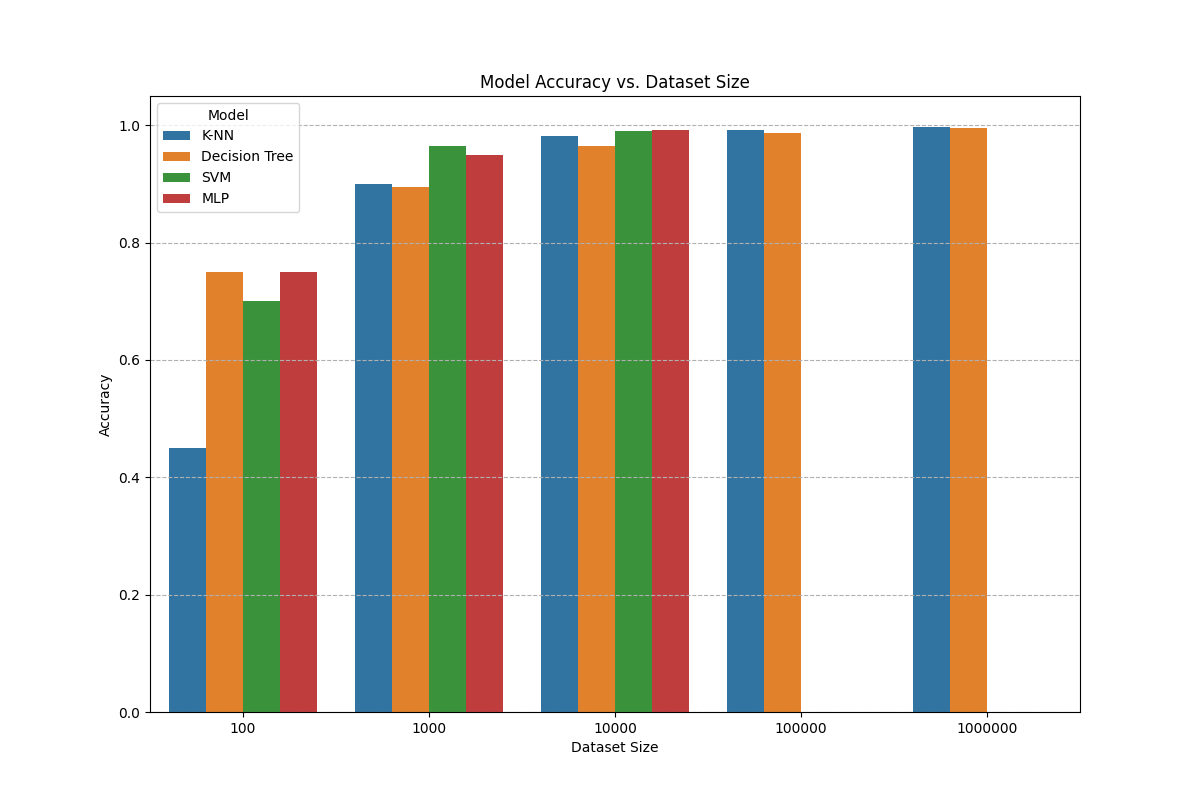
\includegraphics[width=\textwidth]{model_accuracy_vs_dataset_size_barplot.png}
    \caption{Desempeño modelos SC2.}
    \label{fig:barplot_sc2}
  \end{figure}

\end{enumerate}

\section{Escenario 3: grandes datasets vs pequeños datasets}
En este escenario, se indica generar un dataset binario y construir a partir de el dos nuevos datasets, cada uno 
con una tasa de corrupción específica. Las tasas de corrupción definidas son las siguientes: 10\%, y 30\%. De tal forma, 
que en total se tienen 3 datasets, el original y los dos corrompidos de acuerdo con su respectiva tasa de corrupción. El 
\texttt{Assignment \#4} no definió el tamaño de los datasets, así que se optó por conformarlos con 700 registros cada uno. 
Por otra parte, el \texttt{Assignment \#4} si define el tipo de datos que deben tener los datasets, en este caso, de 
tipo \texttt{Moon}. En este escenario tampoco se va a optar por generar un desbalance entre las clases, y tal como se hizo 
en los anteriores, se dividirá cada dataset en conjunto de entrenamiento, validación y prueba, así como la busqueda de los 
mejores hiperparámetros para los mismos modelos de clasificación que se han venido ejecutando. También se tuvo en cuenta 
en la generación de estos datasets, mantener la proporción de clases del dataset original.

\begin{enumerate}

  \item \textbf{k-NN.}
  Probando con un rango de 1 a 30 vecinos (al igual que en los anteriores escenarios) para cada uno de los datasets conformados, 
  se consiguieron las siguientes mejores configuraciones:

  \begin{table}[H]
    \centering
    \small
    \setlength{\tabcolsep}{4pt}
    \begin{tabularx}{\linewidth}{@{}l c c@{}}
      \toprule
      \textbf{Dataset} & \texttt{n\_neighbors}\\
      \midrule
      \texttt{clean}     & 1\\
      \texttt{noisy\_10} & 7\\
      \texttt{noisy\_30} & 25\\
      \bottomrule
    \end{tabularx}
    \caption{Mejores hiperparámetros KNN SC3.}
    \label{tab:best_hparams_knn_sc3}
  \end{table}
  
  Respecto al desempeño obtenido en cada uno de los modelos se tienen los siguientes resultados:

  \small
  \setlength{\tabcolsep}{4pt}
  \begin{longtable}{@{}lcccc@{}}
    \toprule
    \textbf{Clase} & \textbf{Precision} & \textbf{Recall} & \textbf{F1-Score} & \textbf{Support} \\
    \midrule
    \endfirsthead

    \toprule
    \textbf{Clase} & \textbf{Precision} & \textbf{Recall} & \textbf{F1-Score} & \textbf{Support} \\
    \midrule
    \endhead

    \midrule
    \multicolumn{5}{r}{\emph{Continúa en la siguiente página}} \\
    \endfoot

    \bottomrule
    \caption{Reportes de clasificación k-NN SC3.}
    \label{tab:reportes_clasificacion_knn_sc3}
    \endlastfoot

    % ================= clean =================
    \multicolumn{5}{@{}l}{\textbf{(a) clean}}\\
    0 & 1.00 & 1.00 & 1.00 & 70 \\
    1 & 1.00 & 1.00 & 1.00 & 70 \\
    \midrule
    \multicolumn{3}{l}{\textbf{Accuracy}}     & \textbf{1.00} & 140 \\
    \textbf{Macro avg}    & 1.00 & 1.00 & 1.00 & 140 \\
    \textbf{Weighted avg} & 1.00 & 1.00 & 1.00 & 140 \\
    \addlinespace[0.8em]

    % ================= noisy_10 =================
    \multicolumn{5}{@{}l}{\textbf{(b) noisy\_10}}\\
    0 & 0.92 & 0.86 & 0.89 & 71 \\
    1 & 0.86 & 0.93 & 0.90 & 69 \\
    \midrule
    \multicolumn{3}{l}{\textbf{Accuracy}}     & \textbf{0.89} & 140 \\
    \textbf{Macro avg}    & 0.89 & 0.89 & 0.89 & 140 \\
    \textbf{Weighted avg} & 0.89 & 0.89 & 0.89 & 140 \\
    \addlinespace[0.8em]

    % ================= noisy_30 =================
    \multicolumn{5}{@{}l}{\textbf{(c) noisy\_30}}\\
    0 & 0.69 & 0.70 & 0.69 & 69 \\
    1 & 0.70 & 0.69 & 0.70 & 71 \\
    \midrule
    \multicolumn{3}{l}{\textbf{Accuracy}}     & \textbf{0.69} & 140 \\
    \textbf{Macro avg}    & 0.69 & 0.69 & 0.69 & 140 \\
    \textbf{Weighted avg} & 0.69 & 0.69 & 0.69 & 140 \\
  \end{longtable}

  \item \textbf{Arbol de decisión.}
  Se buscó la mejor configuración de hiperparámetros en el mismo marco de los anteriores escenarios (ver \Cref{tab:param_dt_sc1}). Con 
  base en esta busqueda se obtuvieron las siguientes mejores configuraciones de hiperparámetros para cada dataset:

  \begin{table}[htbp]
    \centering\small
    \setlength{\tabcolsep}{4pt}
    \begin{tabularx}{\linewidth}{@{}l c c c c@{}}
      \toprule
      \textbf{Dataset} & \texttt{max\_depth} & \texttt{min\_samples\_leaf} & \texttt{min\_samples\_split}\\
      \midrule
      \texttt{clean}     & \texttt{None} & 1 & 2\\
      \texttt{noisy\_10} & 5             & 2 & 2\\
      \texttt{noisy\_30} & 5             & 4 & 2\\
      \bottomrule
    \end{tabularx}
    \caption{Mejores hiperparámetros Árbol de decisión SC3.}
    \label{tab:best_hparams_dt_sc3}
  \end{table}

  Respecto al desempeño obtenido en cada uno de los modelos se tienen los siguientes resultados:

  \small
  \setlength{\tabcolsep}{4pt}
  \begin{longtable}{@{}lcccc@{}}
    \toprule
    \textbf{Clase} & \textbf{Precision} & \textbf{Recall} & \textbf{F1-Score} & \textbf{Support} \\
    \midrule
    \endfirsthead

    \toprule
    \textbf{Clase} & \textbf{Precision} & \textbf{Recall} & \textbf{F1-Score} & \textbf{Support} \\
    \midrule
    \endhead

    \midrule
    \multicolumn{5}{r}{\emph{Continúa en la siguiente página}} \\
    \endfoot

    \bottomrule
    \caption{Reportes de clasificación Árbol de decisión SC3.}
    \label{tab:reportes_clasificacion_dt_sc3}
    \endlastfoot

    % ================= clean =================
    \multicolumn{5}{@{}l}{\textbf{(a) clean}}\\
    0 & 1.00 & 1.00 & 1.00 & 70 \\
    1 & 1.00 & 1.00 & 1.00 & 70 \\
    \midrule
    \multicolumn{3}{l}{\textbf{Accuracy}}     & \textbf{1.00} & 140 \\
    \textbf{Macro avg}    & 1.00 & 1.00 & 1.00 & 140 \\
    \textbf{Weighted avg} & 1.00 & 1.00 & 1.00 & 140 \\
    \addlinespace[0.8em]

    % ================= noisy_10 =================
    \multicolumn{5}{@{}l}{\textbf{(b) noisy\_10}}\\
    0 & 0.90 & 0.86 & 0.88 & 71 \\
    1 & 0.86 & 0.90 & 0.88 & 69 \\
    \midrule
    \multicolumn{3}{l}{\textbf{Accuracy}}     & \textbf{0.88} & 140 \\
    \textbf{Macro avg}    & 0.88 & 0.88 & 0.88 & 140 \\
    \textbf{Weighted avg} & 0.88 & 0.88 & 0.88 & 140 \\
    \addlinespace[0.8em]

    % ================= noisy_30 =================
    \multicolumn{5}{@{}l}{\textbf{(c) noisy\_30}}\\
    0 & 0.63 & 0.59 & 0.61 & 69 \\
    1 & 0.63 & 0.66 & 0.64 & 71 \\
    \midrule
    \multicolumn{3}{l}{\textbf{Accuracy}}     & \textbf{0.63} & 140 \\
    \textbf{Macro avg}    & 0.63 & 0.63 & 0.63 & 140 \\
    \textbf{Weighted avg} & 0.63 & 0.63 & 0.63 & 140 \\
  \end{longtable}

  \item \textbf{SVM.}
  Para este clasificador se buscó la mejor configuración de hiperparámetros probando los mismos valores del 
  anterior escenario (ver \Cref{tab:param_svm_sc2}). Los mejores hiperparámetros encontrados para cada dataset, 
  fueron los siguientes:

  \begin{table}[htbp]
    \centering\small
    \setlength{\tabcolsep}{4pt}
    \begin{tabularx}{\linewidth}{@{}l c c l c@{}}
      \toprule
      \textbf{Dataset} & \texttt{C} & \texttt{gamma} & \texttt{kernel} \\
      \midrule
      \texttt{clean}     & 1 & \texttt{scale} & \texttt{rbf}\\
      \texttt{noisy\_10} & 1 & \texttt{scale} & \texttt{rbf}\\
      \texttt{noisy\_30} & 1 & \texttt{scale} & \texttt{rbf}\\
      \bottomrule
    \end{tabularx}
    \caption{Mejores hiperparámetros encontrados para SVM SC3.}
    \label{tab:best_hparams_svm_sc3}
  \end{table}
  
  Con los mejores hiperparámetros encontrados, se obtuvieron los siguientes resultados:

  \small
  \setlength{\tabcolsep}{4pt}
  \begin{longtable}{@{}lcccc@{}}
    \toprule
    \textbf{Clase} & \textbf{Precision} & \textbf{Recall} & \textbf{F1-Score} & \textbf{Support} \\
    \midrule
    \endfirsthead

    \toprule
    \textbf{Clase} & \textbf{Precision} & \textbf{Recall} & \textbf{F1-Score} & \textbf{Support} \\
    \midrule
    \endhead

    \midrule
    \multicolumn{5}{r}{\emph{Continúa en la siguiente página}} \\
    \endfoot

    \bottomrule
    \caption{Reportes de clasificación SVM SC3.}
    \label{tab:reportes_clasificacion_svm_sc3}
    \endlastfoot

    % ================= clean =================
    \multicolumn{5}{@{}l}{\textbf{(a) clean}}\\
    0 & 1.00 & 1.00 & 1.00 & 70 \\
    1 & 1.00 & 1.00 & 1.00 & 70 \\
    \midrule
    \multicolumn{3}{l}{\textbf{Accuracy}}     & \textbf{1.00} & 140 \\
    \textbf{Macro avg}    & 1.00 & 1.00 & 1.00 & 140 \\
    \textbf{Weighted avg} & 1.00 & 1.00 & 1.00 & 140 \\
    \addlinespace[0.8em]

    % ================= noisy_10 =================
    \multicolumn{5}{@{}l}{\textbf{(b) noisy\_10}}\\
    0 & 0.92 & 0.86 & 0.89 & 71 \\
    1 & 0.86 & 0.93 & 0.90 & 69 \\
    \midrule
    \multicolumn{3}{l}{\textbf{Accuracy}}     & \textbf{0.89} & 140 \\
    \textbf{Macro avg}    & 0.89 & 0.89 & 0.89 & 140 \\
    \textbf{Weighted avg} & 0.89 & 0.89 & 0.89 & 140 \\
    \addlinespace[0.8em]

    % ================= noisy_30 =================
    \multicolumn{5}{@{}l}{\textbf{(c) noisy\_30}}\\
    0 & 0.69 & 0.70 & 0.69 & 69 \\
    1 & 0.70 & 0.69 & 0.70 & 71 \\
    \midrule
    \multicolumn{3}{l}{\textbf{Accuracy}} & \textbf{0.69} & 140 \\
    \textbf{Macro avg}    & 0.69 & 0.69 & 0.69 & 140 \\
    \textbf{Weighted avg} & 0.69 & 0.69 & 0.69 & 140 \\
  \end{longtable}

   \item \textbf{MLP.}
   Para este clasificador se buscó la mejor configuración de hiperparámetros probando con los siguientes valores:

  \begin{table}[H]
    \centering\small
    \setlength{\tabcolsep}{6pt}
    \begin{tabularx}{\linewidth}{@{}l l X@{}}
      \toprule
      \textbf{Parámetro} & \textbf{Descripción} & \textbf{Valores de búsqueda} \\
      \midrule
      \texttt{hidden\_layer\_sizes} & Tamaño(s) de la(s) capa(s) oculta(s) & \texttt{(50,)}, \texttt{(100,)}, \texttt{(50, 50)} \\
      \texttt{activation}           & Función de activación en capas ocultas & \texttt{tanh}, \texttt{relu} \\
      \texttt{solver}               & Optimizador para los pesos              & \texttt{adam} \\
      \texttt{alpha}                & Penalización L2 (regularización)        & 0.0001, 0.001 \\
      \texttt{learning\_rate\_init} & Tasa de aprendizaje inicial             & 0.001, 0.01 \\
      \bottomrule
    \end{tabularx}
    \caption{Espacio de búsqueda de hiperparámetros para \texttt{MLPClassifier}.}
    \label{tab:param_grid_mlp}
  \end{table}

   Solo se usó un solo optimizador de pesos, conforme lo sugirió la IA de Colab. Con base en esta busqueda se obtuvieron 
   las siguientes mejores configuraciones de hiperparámetros para cada dataset:

  \begin{table}[htbp]
    \centering\small
    \setlength{\tabcolsep}{4pt}
    \begin{tabularx}{\linewidth}{@{}l l l l c c c c@{}}
      \toprule
      \textbf{Dataset} & \texttt{hidden\_layer\_sizes} & \texttt{activation} & \texttt{solver} & \texttt{alpha} & \texttt{learning\_rate\_init} & \texttt{max\_iter}\\
      \midrule
      \texttt{clean}     & \texttt{(50,)}    & \texttt{tanh} & \texttt{adam} & 0.0001 & 0.01  & 200\\
      \texttt{noisy\_10} & \texttt{(50, 50)} & \texttt{tanh} & \texttt{adam} & 0.001  & 0.01  & 500\\
      \texttt{noisy\_30} & \texttt{(50, 50)} & \texttt{relu} & \texttt{adam} & 0.001  & 0.01  & 200\\
      \bottomrule
    \end{tabularx}
    \caption{Mejores hiperparámetros encontrados para MLP SC3.}
    \label{tab:best_hparams_mlp_sc3}
  \end{table}

   Con la configuraciones de hiperparámetros encontradas, se obtuvieron los siguientes resultados:

  \small
  \setlength{\tabcolsep}{4pt}
  \begin{longtable}{@{}lcccc@{}}
    \toprule
    \textbf{Clase} & \textbf{Precision} & \textbf{Recall} & \textbf{F1-Score} & \textbf{Support} \\
    \midrule
    \endfirsthead

    \toprule
    \textbf{Clase} & \textbf{Precision} & \textbf{Recall} & \textbf{F1-Score} & \textbf{Support} \\
    \midrule
    \endhead

    \midrule
    \multicolumn{5}{r}{\emph{Continúa en la siguiente página}} \\
    \endfoot

    \bottomrule
    \caption{Reportes de clasificación del MLP SC3.}
    \label{tab:reportes_clasificacion_mlp_sc3}
    \endlastfoot

    % ================= clean =================
    \multicolumn{5}{@{}l}{\textbf{(a) clean}}\\
    0 & 0.93 & 0.89 & 0.91 & 70 \\
    1 & 0.89 & 0.93 & 0.91 & 70 \\
    \midrule
    \multicolumn{3}{l}{\textbf{Accuracy}}     & \textbf{0.91} & 140 \\
    \textbf{Macro avg}    & 0.91 & 0.91 & 0.91 & 140 \\
    \textbf{Weighted avg} & 0.91 & 0.91 & 0.91 & 140 \\
    \addlinespace[0.8em]

    % ================= noisy_10 =================
    \multicolumn{5}{@{}l}{\textbf{(b) noisy\_10}}\\
    0 & 0.81 & 0.79 & 0.80 & 71 \\
    1 & 0.79 & 0.81 & 0.80 & 69 \\
    \midrule
    \multicolumn{3}{l}{\textbf{Accuracy}}     & \textbf{0.8} & 140 \\
    \textbf{Macro avg}    & 0.80 & 0.80 & 0.80 & 140 \\
    \textbf{Weighted avg} & 0.80 & 0.80 & 0.80 & 140 \\
    \addlinespace[0.8em]

    % ================= noisy_30 =================
    \multicolumn{5}{@{}l}{\textbf{(c) noisy\_30}}\\
    0 & 0.70 & 0.67 & 0.68 & 69 \\
    1 & 0.69 & 0.72 & 0.70 & 71 \\
    \midrule
    \multicolumn{3}{l}{\textbf{Accuracy}}     & \textbf{0.69} & 140 \\
    \textbf{Macro avg}    & 0.69 & 0.69 & 0.69 & 140 \\
    \textbf{Weighted avg} & 0.69 & 0.69 & 0.69 & 140 \\
  \end{longtable}

  \item \textbf{Análisis de resultados.}
  
  En este escenario, el aspecto clave a analizar fue el ruido introducido en las etiquetas de etiquetas: con datos limpios, 
  los cuatro modelos demarcan una frontera nítida y aciertan prácticamente todo, con 10\% de ruido el desempeño baja de forma 
  moderada y los mejores ajustes “se suavizan”, con 30\% de ruido la caída es notoria y los modelos convergen a resultados medios 
  porque la señal contiene contradicciones. En estos casos ayudan más la regularización y márgenes amplios (SVM/MLP), el suavizado 
  en k-NN y el control de profundidad del Árbol.

  La \Cref{fig:barplot_sc3} muestra el desempeño de los modelos ejecutados.

  \begin{figure}[H]
    \centering
    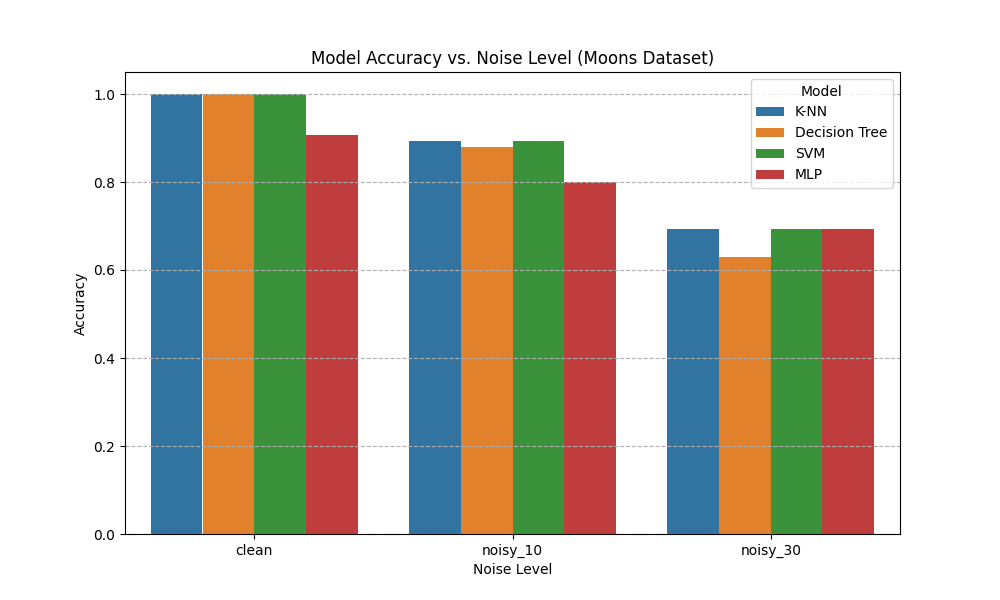
\includegraphics[width=\textwidth]{model_accuracy_vs_noise_level_barplot.png}
    \caption{Desempeño modelos SC3.}
    \label{fig:barplot_sc3}
  \end{figure}

  \end{enumerate}

\section{Discusión de nuestro reciente trabajo sobre LLM}
Elegí el artículo \href{https://arxiv.org/pdf/2507.22900v2}{New Kid in the Classroom: Exploring Student 
Perceptions of AI Coding Assistants} con base en que soy un desarrollador de software que recientemente 
empezó a desarrollar, y por lo tanto, no me he formado en esta área sin la existencia y asistencia de la 
Inteligencia Artificial (IA), me gustaría indagar como se puede hacer uso de la IA de una manera propiada 
sin incurrir en una dependencia de la IA, o en no aprender apropiadamente los conceptos. A continuación, 
dejo mis impresiones sobre lo que considero podrían ser nuevas propuestas de investigación con base en la 
lectura del artículo mencionado.

\begin{enumerate}
  \item \textbf{Análisis del aprendizaje con IA.} 
  \textit{Hipótesis:} la IA acelera el aprendizaje inicial, pero puede reducir la verdadera captura y 
  retención del conocimiento cuando se retira. 

  \item \textbf{Como pensar con la IA.} 
  \textit{Hipótesis:} guiar el uso de IA hacia la explicación, la crítica y las preguntas, mejora la 
  comprensión y autonomía frente a la simple solicitud de tareas. 
\end{enumerate}
\end{document}
